\documentclass[]{standalone}

\usepackage{scalefnt}
\usepackage{tikz}  
\usepackage{tikz-3dplot} 
\usepackage{amssymb,amsfonts,amsmath}
\usepackage{tikz,tkz-euclide}
\usetikzlibrary{arrows,calc,patterns}


\begin{document}
\scalefont{0.5}
    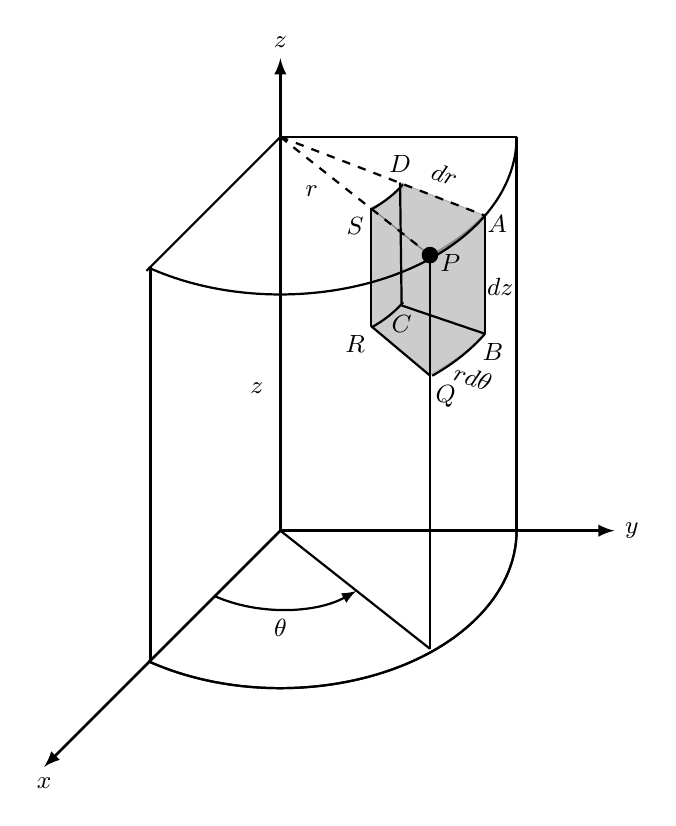
\begin{tikzpicture}[]
    \tikzstyle{every node}=[font=\small]
      \coordinate (O)  at (0,0);
      \coordinate (Ox) at (-3,-3);
      \coordinate (Oy) at (4.243,0);  % sqrt{18}
      \coordinate (Oz) at (0, 6);

      % draw axis 
      \draw[-latex, line width=1] (O)-- (Ox) node[below] {$x$};
      \draw[-latex, line width=1] (O)-- (Oy) node[right] {$y$};
      \draw[-latex, line width=1] (O)-- (Oz) node[above] {$z$};


      % draw arcs
       \draw[thick] ($(0, 0) + (236:3cm and 2cm)$(P) arc
         (236:360:3cm and 2cm);
       \draw[thick] ($(0, 0) + (236:3cm and 2cm)$(P) arc
         (236:360:3cm and 2cm);

       \draw[thick] ($(0, 5) + (236:3cm and 2cm)$(P) arc
         (236:360:3cm and 2cm);

       \draw[thick, -latex] ($(0, 0) + (236:1.5cm and 1cm)$(P) arc
         (236:310:1.5cm and 1cm);

         \coordinate (Phi) at (0,-1) ;
         \node[below] at (Phi) {$\theta$};

    	 \coordinate (Rad) at (.4,4.5) ;
         \node[below] at (Rad) {$r$};
         \node[below] at (-0.3,2) {$z$};

      \coordinate (A1) at (0, 5);
      \coordinate (B) at (3, 5);
      \coordinate (C) at (-1.7, 3.3);
      \draw[thick] (A1)--(B);
      \draw[thick] (A1)--(C);

      % radius
      \coordinate (D) at (1.9,-1.5);
      \coordinate (P) at (1.9,3.5);
      \draw[thick] (O)--(D);
      \draw[thick, dashed] (A1)--(P) node[right, yshift=-1mm] {$P$};
      \draw[thick] (D)--(P);
      \fill[black] (P) circle (3pt);


      \coordinate (A) at (2.6, 4.0);
      \draw[thick, dashed] (A1)--(A) node[right, yshift=-1mm, xshift=-1mm] {$A$};


      % arcs
       \draw[thick] ($(0, 5) + (310:1.8cm and 1.2cm)$(P) arc
         (310:330:1.8cm and 1.2cm);

       \draw[thick] ($(0, 3.5) + (310:1.8cm and 1.2cm)$(P) arc
         (310:330:1.8cm and 1.2cm);

       \draw[thick] ($(0, 3.5) + (310:3cm and 2cm)$(P) arc
         (310:330:3cm and 2cm);

       \coordinate (Q) at (1.9,1.97);
       \node[below,xshift=2mm] at (Q) {$Q$};
        % \fill[black] (Q) circle (3pt);


      \coordinate (B) at (2.6, 2.5);
      \node[below,xshift=1mm] at (B) {$B$};
       % \fill[black] (B) circle (3pt);
      \draw[thick] (A) --(B);

      \coordinate (S) at (1.15, 4.1);
      \node[below, xshift=-2mm] at (S) {$S$};
       % \fill[black] (S) circle (3pt);

      \coordinate (R) at (1.15, 2.6);
      \node[below, xshift=-2mm] at (R) {$R$};
       %\fill[black] (R) circle (3pt);


      \coordinate (D) at (1.52, 4.42);
      \node[above] at (D) {$D$};
      % \fill[black] (D) circle (3pt);

      \coordinate (C) at (1.54, 2.86);
      \node[below] at (C) {$C$};
      %\fill[black] (C) circle (3pt);

      \draw[thick] (S) --(R);
      \draw[thick] (D) --(C);
      \draw[thick] (R) --(Q);
      \draw[thick] (C) --(B);

      % verticals on the planes
      \coordinate (H) at (-1.65,-1.65);
      %\fill[black] (H) circle (3pt);
      %
      \coordinate (I) at (-1.65,3.35);
      %\fill[black] (I) circle (3pt);
      \draw[thick] (H) --(I);

      \coordinate (J) at (3,0);
      %\fill[black] (J) circle (3pt);
      \coordinate (K) at (3,5);
      %\fill[black] (K) circle (3pt);
      \draw[thick] (J) --(K);

      % filling
      \filldraw[opacity=0.2]
          (D)--(A) arc (325:306:3cm and 2.2cm)--(S)
           arc (305:325:1.8cm and 1.2cm)--cycle;

      \filldraw[opacity=0.2]
          (P) arc (306:325:3cm and 2.2cm)--(B)
           arc (325:306:3.0cm and 2.2cm)--cycle;

       \filldraw[opacity=0.2]
         (P)--(Q)--(R)--(S)--cycle;

      % differential labels
      \node[right, yshift=1mm,xshift=2mm, rotate=-20] at (Q) {$r d \theta$};
      \node[right, yshift=6mm, xshift=-1mm ] at (B) {$dz$};
      \node[right,xshift=3mm, yshift=2mm, rotate=-20] at (D) {$dr$};

    \end{tikzpicture}

\end{document}